% Options for packages loaded elsewhere
\PassOptionsToPackage{unicode}{hyperref}
\PassOptionsToPackage{hyphens}{url}
%
\documentclass[
  english,
  man,mask,floatsintext]{apa6}
\usepackage{amsmath,amssymb}
\usepackage{lmodern}
\usepackage{ifxetex,ifluatex}
\ifnum 0\ifxetex 1\fi\ifluatex 1\fi=0 % if pdftex
  \usepackage[T1]{fontenc}
  \usepackage[utf8]{inputenc}
  \usepackage{textcomp} % provide euro and other symbols
\else % if luatex or xetex
  \usepackage{unicode-math}
  \defaultfontfeatures{Scale=MatchLowercase}
  \defaultfontfeatures[\rmfamily]{Ligatures=TeX,Scale=1}
\fi
% Use upquote if available, for straight quotes in verbatim environments
\IfFileExists{upquote.sty}{\usepackage{upquote}}{}
\IfFileExists{microtype.sty}{% use microtype if available
  \usepackage[]{microtype}
  \UseMicrotypeSet[protrusion]{basicmath} % disable protrusion for tt fonts
}{}
\makeatletter
\@ifundefined{KOMAClassName}{% if non-KOMA class
  \IfFileExists{parskip.sty}{%
    \usepackage{parskip}
  }{% else
    \setlength{\parindent}{0pt}
    \setlength{\parskip}{6pt plus 2pt minus 1pt}}
}{% if KOMA class
  \KOMAoptions{parskip=half}}
\makeatother
\usepackage{xcolor}
\IfFileExists{xurl.sty}{\usepackage{xurl}}{} % add URL line breaks if available
\IfFileExists{bookmark.sty}{\usepackage{bookmark}}{\usepackage{hyperref}}
\hypersetup{
  pdftitle={Understanding demographic predictors and academic outcomes of active and passive VLE engagement},
  pdfauthor={First Author1 \& Ernst-August Doelle1,2},
  pdflang={en-EN},
  pdfkeywords={learning analytics, virtual learning environments, online teaching},
  hidelinks,
  pdfcreator={LaTeX via pandoc}}
\urlstyle{same} % disable monospaced font for URLs
\usepackage{graphicx}
\makeatletter
\def\maxwidth{\ifdim\Gin@nat@width>\linewidth\linewidth\else\Gin@nat@width\fi}
\def\maxheight{\ifdim\Gin@nat@height>\textheight\textheight\else\Gin@nat@height\fi}
\makeatother
% Scale images if necessary, so that they will not overflow the page
% margins by default, and it is still possible to overwrite the defaults
% using explicit options in \includegraphics[width, height, ...]{}
\setkeys{Gin}{width=\maxwidth,height=\maxheight,keepaspectratio}
% Set default figure placement to htbp
\makeatletter
\def\fps@figure{htbp}
\makeatother
\setlength{\emergencystretch}{3em} % prevent overfull lines
\providecommand{\tightlist}{%
  \setlength{\itemsep}{0pt}\setlength{\parskip}{0pt}}
\setcounter{secnumdepth}{-\maxdimen} % remove section numbering
% Make \paragraph and \subparagraph free-standing
\ifx\paragraph\undefined\else
  \let\oldparagraph\paragraph
  \renewcommand{\paragraph}[1]{\oldparagraph{#1}\mbox{}}
\fi
\ifx\subparagraph\undefined\else
  \let\oldsubparagraph\subparagraph
  \renewcommand{\subparagraph}[1]{\oldsubparagraph{#1}\mbox{}}
\fi
% Manuscript styling
\usepackage{upgreek}
\captionsetup{font=singlespacing,justification=justified}

% Table formatting
\usepackage{longtable}
\usepackage{lscape}
% \usepackage[counterclockwise]{rotating}   % Landscape page setup for large tables
\usepackage{multirow}		% Table styling
\usepackage{tabularx}		% Control Column width
\usepackage[flushleft]{threeparttable}	% Allows for three part tables with a specified notes section
\usepackage{threeparttablex}            % Lets threeparttable work with longtable

% Create new environments so endfloat can handle them
% \newenvironment{ltable}
%   {\begin{landscape}\centering\begin{threeparttable}}
%   {\end{threeparttable}\end{landscape}}
\newenvironment{lltable}{\begin{landscape}\centering\begin{ThreePartTable}}{\end{ThreePartTable}\end{landscape}}

% Enables adjusting longtable caption width to table width
% Solution found at http://golatex.de/longtable-mit-caption-so-breit-wie-die-tabelle-t15767.html
\makeatletter
\newcommand\LastLTentrywidth{1em}
\newlength\longtablewidth
\setlength{\longtablewidth}{1in}
\newcommand{\getlongtablewidth}{\begingroup \ifcsname LT@\roman{LT@tables}\endcsname \global\longtablewidth=0pt \renewcommand{\LT@entry}[2]{\global\advance\longtablewidth by ##2\relax\gdef\LastLTentrywidth{##2}}\@nameuse{LT@\roman{LT@tables}} \fi \endgroup}

% \setlength{\parindent}{0.5in}
% \setlength{\parskip}{0pt plus 0pt minus 0pt}

% \usepackage{etoolbox}
\makeatletter
\patchcmd{\HyOrg@maketitle}
  {\section{\normalfont\normalsize\abstractname}}
  {\section*{\normalfont\normalsize\abstractname}}
  {}{\typeout{Failed to patch abstract.}}
\patchcmd{\HyOrg@maketitle}
  {\section{\protect\normalfont{\@title}}}
  {\section*{\protect\normalfont{\@title}}}
  {}{\typeout{Failed to patch title.}}
\makeatother
\shorttitle{Predictors and outcomes of VLE engagement}
\keywords{learning analytics, virtual learning environments, online teaching\newline\indent Word count: 1998}
\usepackage{csquotes}
\ifxetex
  % Load polyglossia as late as possible: uses bidi with RTL langages (e.g. Hebrew, Arabic)
  \usepackage{polyglossia}
  \setmainlanguage[]{english}
\else
  \usepackage[main=english]{babel}
% get rid of language-specific shorthands (see #6817):
\let\LanguageShortHands\languageshorthands
\def\languageshorthands#1{}
\fi
\ifluatex
  \usepackage{selnolig}  % disable illegal ligatures
\fi
\newlength{\cslhangindent}
\setlength{\cslhangindent}{1.5em}
\newlength{\csllabelwidth}
\setlength{\csllabelwidth}{3em}
\newenvironment{CSLReferences}[2] % #1 hanging-ident, #2 entry spacing
 {% don't indent paragraphs
  \setlength{\parindent}{0pt}
  % turn on hanging indent if param 1 is 1
  \ifodd #1 \everypar{\setlength{\hangindent}{\cslhangindent}}\ignorespaces\fi
  % set entry spacing
  \ifnum #2 > 0
  \setlength{\parskip}{#2\baselineskip}
  \fi
 }%
 {}
\usepackage{calc}
\newcommand{\CSLBlock}[1]{#1\hfill\break}
\newcommand{\CSLLeftMargin}[1]{\parbox[t]{\csllabelwidth}{#1}}
\newcommand{\CSLRightInline}[1]{\parbox[t]{\linewidth - \csllabelwidth}{#1}\break}
\newcommand{\CSLIndent}[1]{\hspace{\cslhangindent}#1}

\title{Understanding demographic predictors and academic outcomes of active and passive VLE engagement}
\author{First Author\textsuperscript{1} \& Ernst-August Doelle\textsuperscript{1,2}}
\date{}


\authornote{

Add complete departmental affiliations for each author here. Each new line herein must be indented, like this line.

Enter author note here.

The authors made the following contributions. First Author: Conceptualization, Writing - Original Draft Preparation, Writing - Review \& Editing; Ernst-August Doelle: Writing - Review \& Editing.

Correspondence concerning this article should be addressed to First Author, Postal address. E-mail: \href{mailto:my@email.com}{\nolinkurl{my@email.com}}

}

\affiliation{\vspace{0.5cm}\textsuperscript{1} Wilhelm-Wundt-University\\\textsuperscript{2} Konstanz Business School}

\abstract{
Virtual Learning Environments (VLEs) have gained pride of place in university teaching, not just in pandemic times. However, student engagement with the resources offered there appears to be highly unequal. In order to use VLEs effectively, we need to understand whether they contribute to students' achievement and whether inequalities in engagement exacerbate pre-existing inequalities.

Using a large-scale dataset released by the Open University, I analyse the VLE interactions of more than 9,000 students who completed social science modules. In line with expectations, VLE engagement was found to substantially predict assessment grades. Furthermore, it was predicted by students' age and their socioeconomic background. Importantly, differences in VLE engagement appeared to offer a partial explanation for the link between socioeconomic status and assessment outcomes. Contrary to expectations, in the aggregate, there was no evidence that active participation in forums and quizzes was a better predictor of outcomes than (passive) engagement with content pages.

I discuss implications of these findings for the use of VLE environments in my teaching, their limitations and directions for future research.
}



\begin{document}
\maketitle

Most universities have embraced the use of virtual learning environments (VLEs), where learning materials and interaction opportunities are offered to all students studying on a given module. While this preceded the Covid-19 pandemics, the ensuing growth in online and blended teaching made it even more important to understand how students use VLE resources and how they can contribute to learning.

In this paper, I analyse the largest openly available data set that describes students' interactions with online learning environments. The Open University Learning Analytics Dataset (OULAD) was released in 2017 and covers more than 10 million VLE interactions by more than 32,000 students (Kuzilek, Hlosta, \& Zdrahal, 2017). To date, it has been used in dozens of papers, mostly using advanced machine learning methods to predict student progression and retention from large datasets (e.g., Hussain, Zhu, Zhang, \& Abidi, 2018; Waheed et al., 2020). While such research can inform the development of VLE dashboards and other teaching management tools, such approaches tends to be of limited relevance to practitioners who seek guidance regarding the design of the VLE pages for their teaching. In this paper, I attempt to extract such practically relevant insights from the dataset.

\hypertarget{research-questions}{%
\subsection{Research questions}\label{research-questions}}

Specifically, I aim to answer the following questions:

\begin{enumerate}
\def\labelenumi{\arabic{enumi}.}
\tightlist
\item
  Does students' level of engagement with a VLE predict their assessment results?\footnote{Hussain, Zhu, Zhang, and Abidi (2018) have already shown this association to be statistically significant. However, they did not report effect sizes or focus on social science courses.}
\item
  Is there a difference in the observed effects of engaging actively (e.g., in forums) and passively (e.g., by watching videos and reading text)?
\item
  Is VLE engagement linked to students' demographic background, and thus to pre-existing inequalities?
\end{enumerate}

\hypertarget{methods}{%
\section{Methods}\label{methods}}

\hypertarget{participants}{%
\subsection{Participants}\label{participants}}

\begin{figure}
\centering
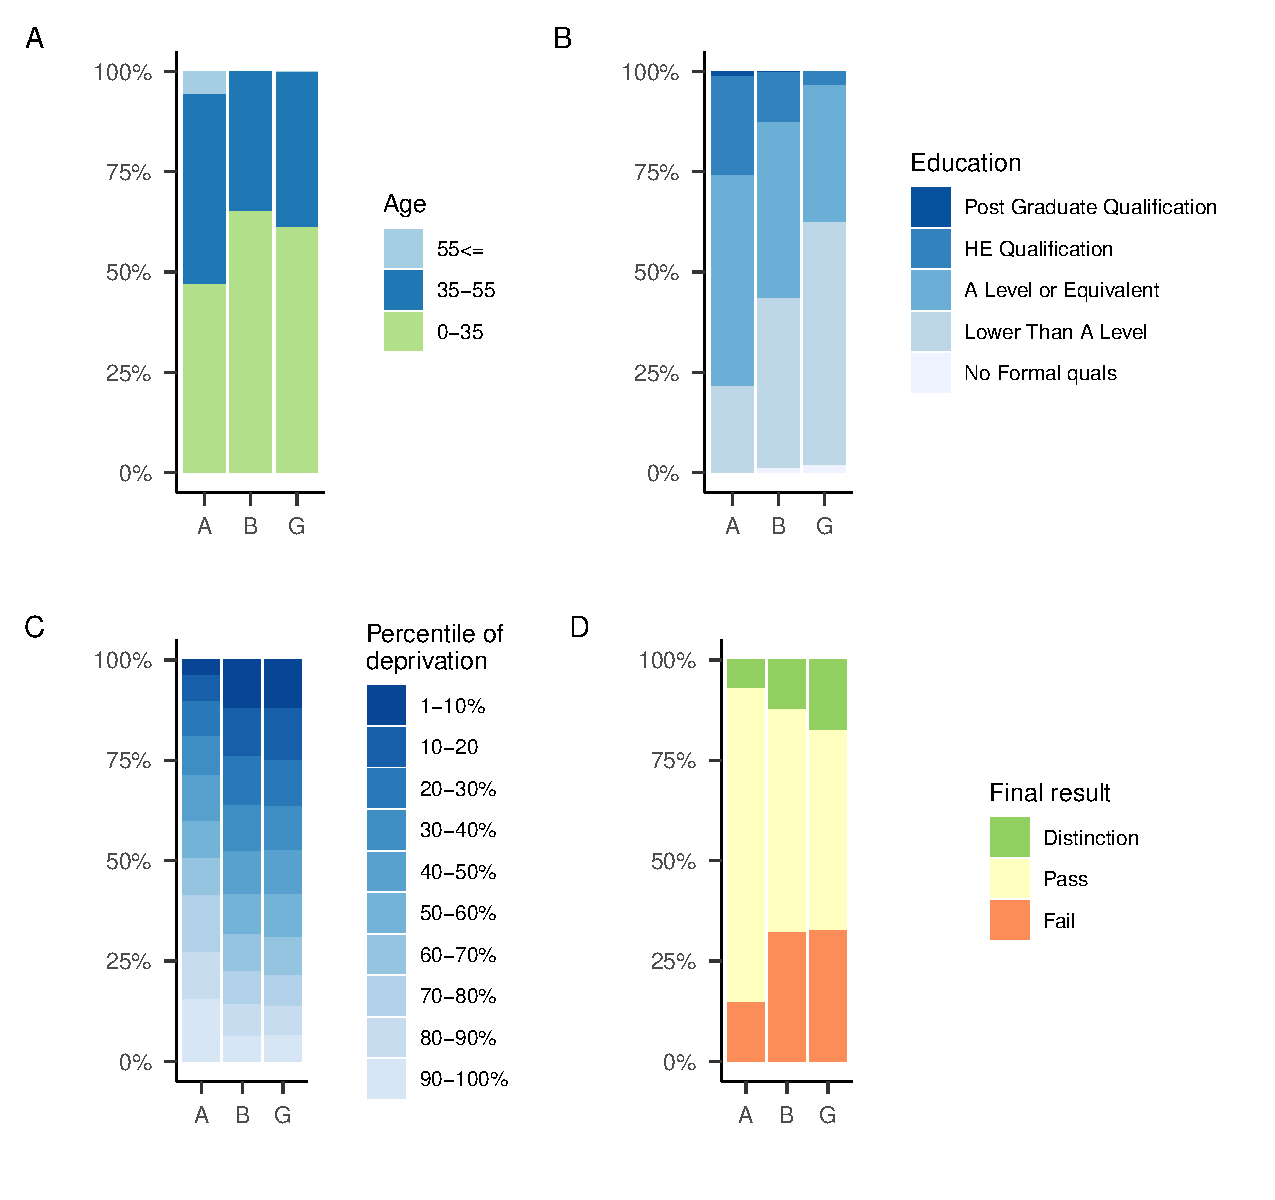
\includegraphics{Assigment-2---OU-data_files/figure-latex/unnamed-chunk-1-1.pdf}
\caption{\label{fig:unnamed-chunk-1}Sample composisition by module and students' age, prior education, local deprivation and final result \label{fig:exp1}}
\end{figure}

Within the OULAD dataset, I only considered Social Science modules, given that these are closer to my teaching reality than the STEM modules also included Also, only students who completed the modules were included to focus on learning rather than retention (for analyses focusing on retention, see Hassan et al., 2019). This restricted the sample to 8330 students (82.7\% female) across three modules. In line with the Open University student body, they were diverse in terms of age, educational qualifications and the level of deprivation of their post code\footnote{This was measured with the index of multiple deprivation that combines seven domains and expressed as percentiles that rank localities from 1 (most deprived) to 100 (least deprived). For details, see Smith et al. (2015).} (see \autoref{fig:exp1}).

\hypertarget{data-analysis-and-code-availability}{%
\subsection{Data analysis and code availability}\label{data-analysis-and-code-availability}}

I used R {[}Version 4.1.0; R Core Team (2021){]} for all analyses and for the preparation of this manuscript.\footnote{I, furthermore, used the R-packages \emph{papaja} {[}Version 0.1.0.9997; Aust and Barth (2020){]}, \emph{patchwork} {[}Version 1.1.1; Pedersen (2020){]}, \emph{tidyverse} {[}Version 1.3.1; Wickham et al. (2019){]}, and \emph{timesaveR} {[}Version 0.0.1.9016; Wallrich (2021){]}.} The full code is shared on GitHub: \href{https://github.com/LukasWallrich/PGCert}{(https://github.com/LukasWallrich/PGCert)}. In general, I analysed relationships separately by module and cohort to see to what extent findings are consistent.

\hypertarget{results}{%
\section{Results}\label{results}}

\hypertarget{description-of-vle-interactions}{%
\subsection{Description of VLE interactions}\label{description-of-vle-interactions}}

\autoref{fig:exp2} illustrates students' average frequency of interactions with different types of VLE pages. Panel A expresses this as the number of days the student interacted with the resource, while Panel B focuses on the number of clicks, thereby also including the intensity of engagement. The results highlight that VLE usage in module A was substantially higher than that in the other two modules, and that in each module, students engaged most intensely with the homepage, forums and OU learning content.

\begin{figure}
\centering
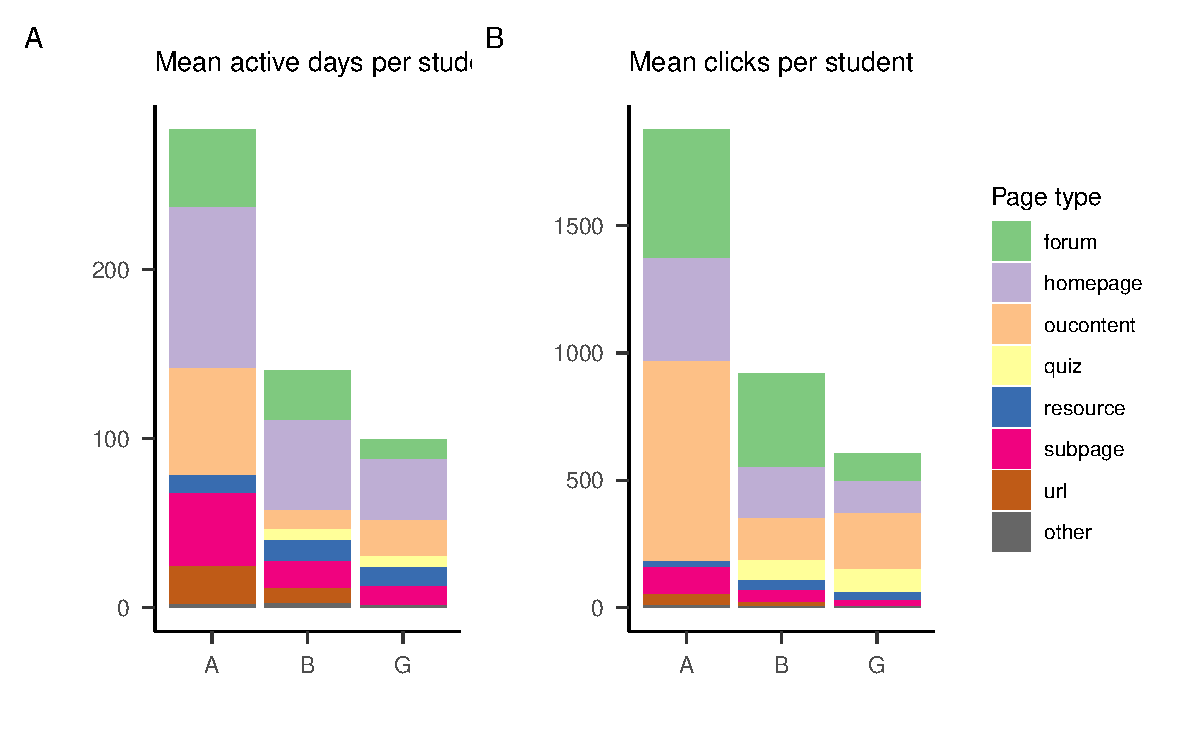
\includegraphics{Assigment-2---OU-data_files/figure-latex/unnamed-chunk-3-1.pdf}
\caption{\label{fig:unnamed-chunk-3}Average frequency of interaction with various types of pages \label{fig:exp2}}
\end{figure}

Students' frequency of engaging with the VLE pages varied drastically. \autoref{fig:exp3} shows the distribution on a logarithmic scale, with equal-sized steps on the y-axis indicating a doubling of the frequency of engagement (reasons for using such scales will be discussed below). The data indicates that across modules, students tended to engage more frequently with resources that focused on passive rather than active learning.\footnote{VLE forums and quizzes were taken to use an active learning mode, while all other pages were considered to focus on passive learning. The homepage for each module is shown separately, given that is is likely to be a gateway to both types of resources.}

\begin{figure}
\centering
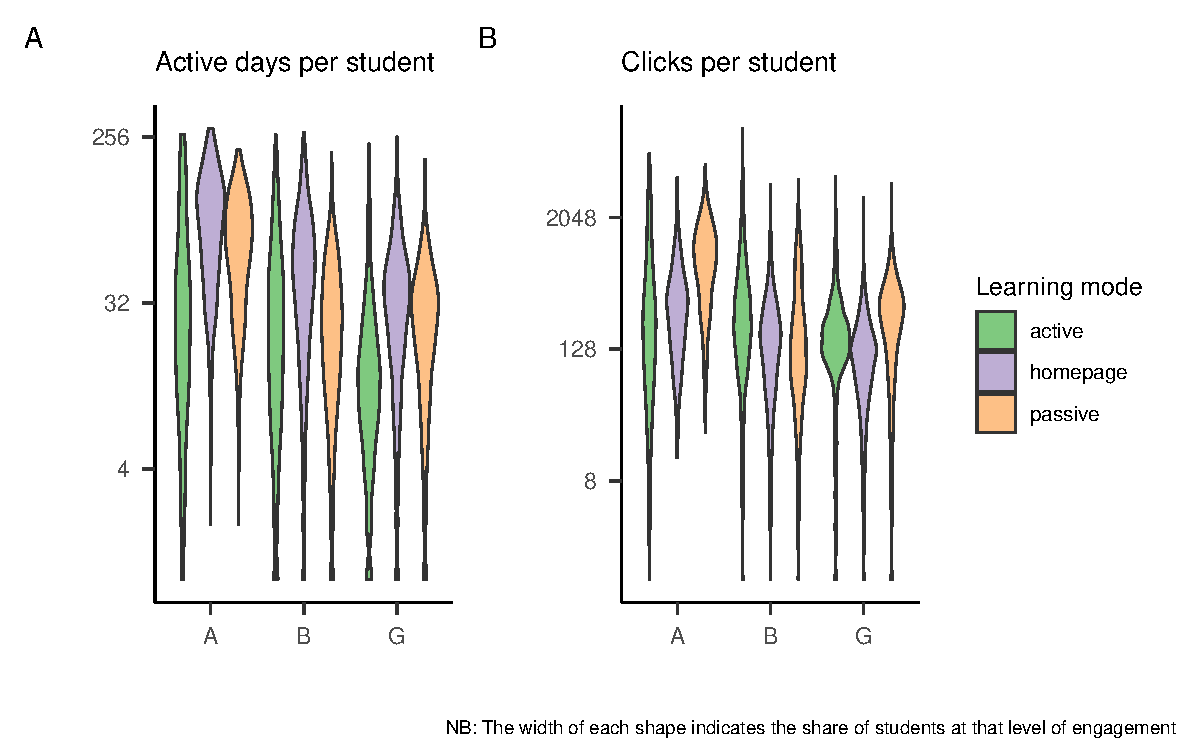
\includegraphics{Assigment-2---OU-data_files/figure-latex/unnamed-chunk-4-1.pdf}
\caption{\label{fig:unnamed-chunk-4}Distribution of interaction frequencies \label{fig:exp3}}
\end{figure}

\hypertarget{engagement-predicts-results}{%
\subsection{Engagement predicts results}\label{engagement-predicts-results}}

Following from these descriptions, I turn to the first research question, namely whether VLE engagement can predict module results. From here, for parsimony, I only report results based on the number of active days as an indicator of engagement; results of models focused on the number of clicks were generally comparable. \autoref{fig:exp4} shows that across modules and cohorts, there was a clear positive relationship between VLE engagement and students' average assessment grade. Here I again use logarithmic scales, for two reasons: technically, logarithmic scales can be used when the data is substantially skewed towards small values, as is the case here, in order to reduce the effect of outliers. More importantly, their use makes substantive sense when there is reason to assume a declining \emph{incremental} effect. Here, it appears very likely that the first day of engagement will contribute more to learning than the 101st day. Therefore, I tested how each doubling of the number of active days is linked to the grade. In \autoref{fig:exp4}, lines are shown that indicate how a General Additive Model (Hastie \& Tibshirani, 1990) estimates the relationship. This does not assume a linear relationship and allows for any curves to be included. However, if the relationship is linear in the areas with the densest clustering of observations, non-linearity beyond might be a result due to over-fitting, i.e.~driven by random variations in the sample. Given that this is the case here, I preferred linear models for the statistical test.

\begin{figure}
\centering
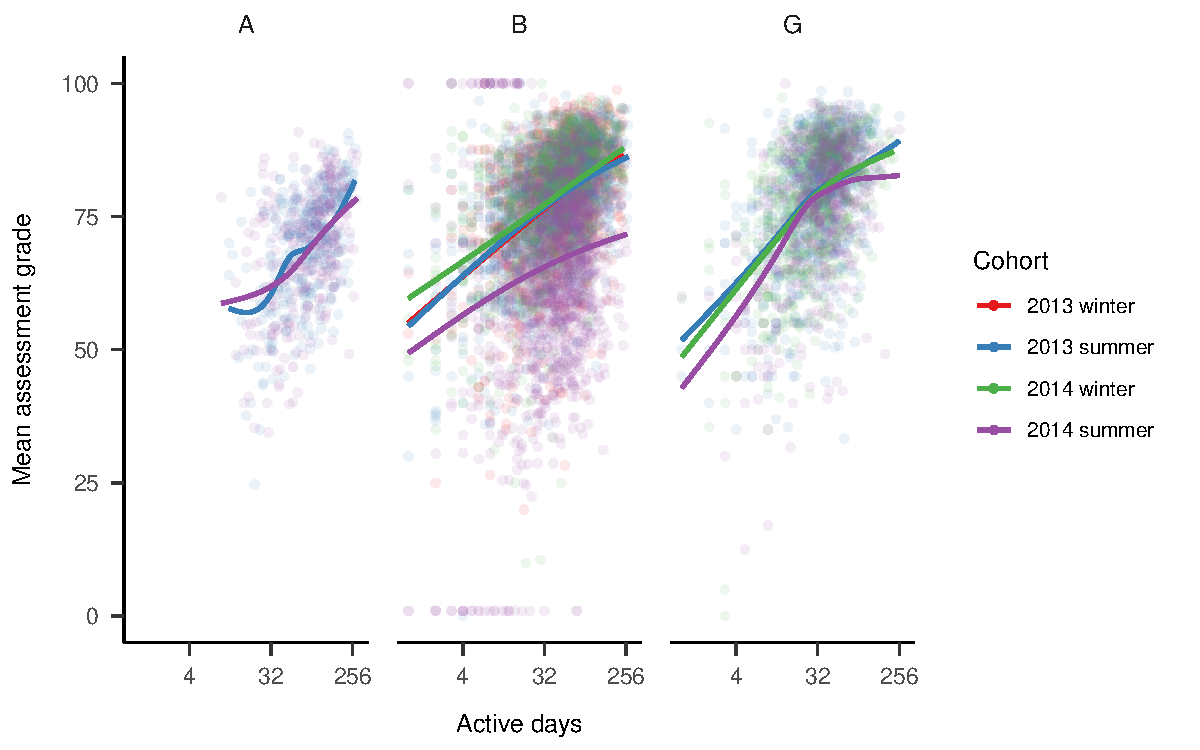
\includegraphics{Assigment-2---OU-data_files/figure-latex/unnamed-chunk-5-1.pdf}
\caption{\label{fig:unnamed-chunk-5}Relationship between VLE activity and assessment results \label{fig:exp4}}
\end{figure}

Linear regression models predicting the average grade from the logarithm of base 2 of the number of active days show that VLE activity consistently significantly predicts average assessment grades, all \emph{p}s \textless{} .0001. Typically, the number of days with VLE activity explained around 20\% of the variance in assessment grades (19.1\% \textless{} \(R^2\) \textless{} 27.4\%), which can be considered a large effect in educational research (Sanders, Chonaire, \& others, 2015). In terms of assessment marks, the gap between those in the upper quartile of VLE engagement and those in the lower quartile was predicted to be more than one grade band (12.3 to 15.6 marks). The only exception to this was the 2014 summer cohort in the B module, with an \(R^2\) of 3.8\% (grade difference of 7.8 marks), where a large number of straight 0 and 100 grades increased the variance of assessment grades. This is more likely to reflect an issue with the data or grading in that module than a divergence of interest to the research questions asked here.

\hypertarget{differences-between-active-and-passive-engagement}{%
\subsubsection{Differences between active and passive engagement}\label{differences-between-active-and-passive-engagement}}

In order to gain some insights into how to best design VLE activities, I tested whether the associations differed depending on whether the engagement took place with active (e.g., forums) or passive (e.g., resource) pages. Visual exploration (see \autoref{fig:exp5}) suggested that both types were positively correlated with assessment grades. Based on the general additive model line, the relationships between the second logarithm of the number of active days and assessment grades can again be plausibly assumed to be linear. Therefore, I estimated linear regression models predicting assessment grades from both active and passive engagement.

\begin{figure}
\centering
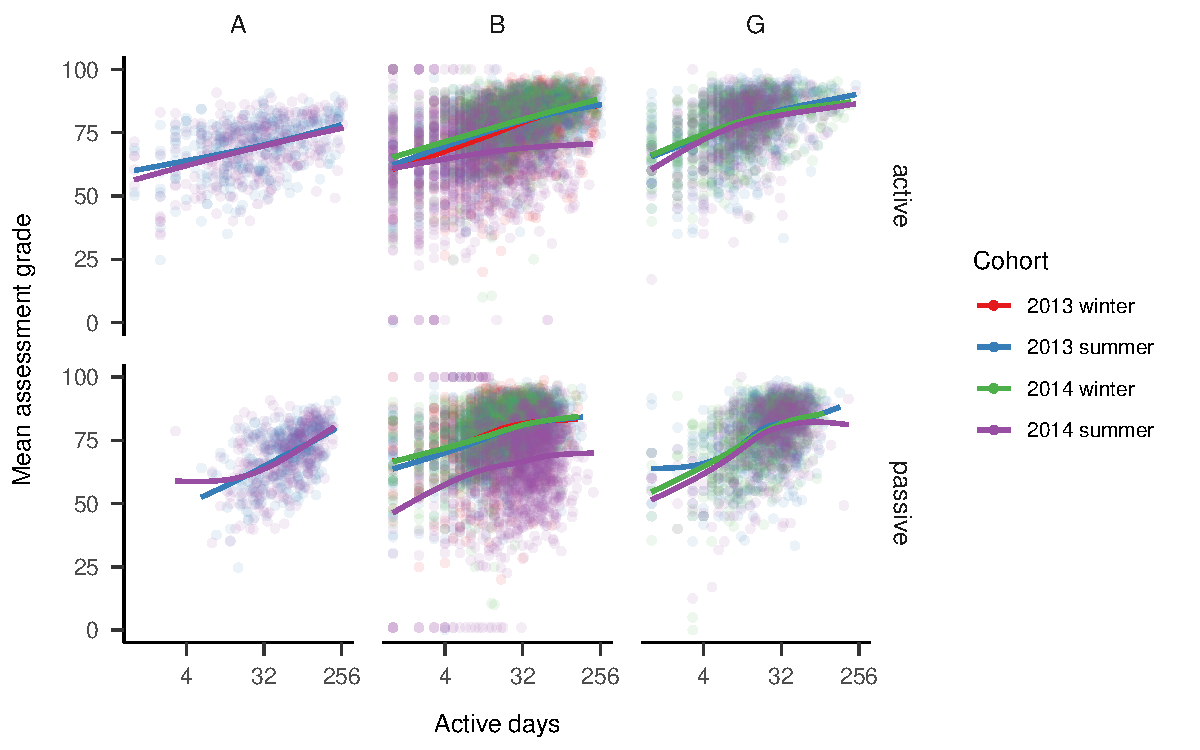
\includegraphics{Assigment-2---OU-data_files/figure-latex/unnamed-chunk-6-1.pdf}
\caption{\label{fig:unnamed-chunk-6}Relationship between VLE activity and assessment results by mode \label{fig:exp5}}
\end{figure}

These models revealed different patterns between the modules (see \autoref{tab:coef}). In module A, passive engagement had a stronger relationship with grades than active engagement did, while active engagement mattered more in module B (except for the summer 2014 cohort, which has already been identified as an outlier). In module G, the differences were not statistically significant, but passive engagement again tended to be the stronger predictor.



\begin{table}[tbp]

\begin{center}
\begin{threeparttable}

\caption{\label{tab:coef}Association of active and passive engagement with assessment grades}

\footnotesize{

\begin{tabular}{lllll}
\toprule
 &  & \multicolumn{2}{c}{Regression coefficients}  &\\
\cmidrule(r){3-4}
Module & \multicolumn{1}{c}{Cohort} & \multicolumn{1}{c}{Active engagement} & \multicolumn{1}{c}{Passive engagement} & \multicolumn{1}{c}{Difference}\\
\midrule
A & 2013 summer & 0.69 & 4.52 & -3.84 ***\\
A & 2014 summer & 0.93 & 4.22 & -3.28 *\\ \midrule
B & 2013 winter & 3.62 & -0.30 & 3.92 ***\\
B & 2013 summer & 2.59 & 0.77 & 1.82 ***\\
B & 2014 winter & 2.73 & 0.35 & 2.38 ***\\
B & 2014 summer & 0.48 & 2.25 & -1.77\\ \midrule
G & 2013 summer & 2.20 & 2.23 & -0.03\\
G & 2014 winter & 1.70 & 2.58 & -0.88\\
G & 2014 summer & 1.53 & 2.92 & -1.39\\
\bottomrule
\addlinespace
\end{tabular}

}

\begin{tablenotes}[para]
\normalsize{\textit{Note.} *** \emph{p} \textless{} .001, ** \emph{p} \textless{} .01, * \emph{p} \textless{} .05 (\emph{p}-values are adjusted for multiple comparisons using the Holm-Bonferroni method.)}
\end{tablenotes}

\end{threeparttable}
\end{center}

\end{table}

\hypertarget{association-between-vle-usage-and-demographics}{%
\subsection{Association between VLE usage and demographics}\label{association-between-vle-usage-and-demographics}}

\begin{table}[tbp]

\begin{center}
\begin{threeparttable}

\caption{\label{tab:dem-vle-associations}Associations between demographic characteristics and VLE engagement}

\footnotesize{

\begin{tabular}{llllllll}
\toprule
 &  & \multicolumn{5}{c}{Predictors}  &\\
\cmidrule(r){3-7}
Module & \multicolumn{1}{c}{Cohort} & \multicolumn{1}{c}{Local Deprivation} & \multicolumn{1}{c}{Highest Education} & \multicolumn{1}{c}{Gender} & \multicolumn{1}{c}{Disability} & \multicolumn{1}{c}{Age Band} & \multicolumn{1}{c}{$R^2$}\\
\midrule
A & 2013 summer & $\checkmark$ &  &  &  & $\checkmark$ & 0.17\\
A & 2014 summer &  &  & $\checkmark$ &  & $\checkmark$ & 0.09\\ \midrule
B & 2013 winter & $\checkmark$ &  &  &  & $\checkmark$ & 0.02\\
B & 2013 summer & $\checkmark$ & $\checkmark$ &  &  & $\checkmark$ & 0.06\\
B & 2014 winter & $\checkmark$ &  &  &  & $\checkmark$ & 0.04\\
B & 2014 summer & $\checkmark$ & $\checkmark$ &  &  & $\checkmark$ & 0.05\\ \midrule
G & 2013 summer & $\checkmark$ &  &  & $\checkmark$ & $\checkmark$ & 0.04\\
G & 2014 winter & $\checkmark$ &  &  & $\checkmark$ & $\checkmark$ & 0.11\\
G & 2014 summer &  &  &  &  & $\checkmark$ & 0.04\\
\bottomrule
\addlinespace
\end{tabular}

}

\begin{tablenotes}[para]
\normalsize{\textit{Note.} Checkmarks indicate that this characteristic predicted VLE engagement significantly.}
\end{tablenotes}

\end{threeparttable}
\end{center}

\end{table}

Given that VLE usage varied widely between students and had a strong association with assessment outcomes, I considered whether VLE usage is related to demographic factors that predict student outcomes. To that effect, I ran linear regression models to see whether student's age category, gender, disability status, or level of previous education predicted their frequency of VLE usage. Overall, only students' age and the level of deprivation in their local postcode consistently predicted VLE engagement, and the demographic predictors typically accounted for less than 10\% of the variance in VLE usage (see \autoref{tab:dem-vle-associations}).

In spite of these relatively small associations, this suggests that differences in VLE engagement might help explain how demographic inequalities come to shape academic outcomes. As \autoref{fig:exp6} shows, a greater level of deprivation was typically associated with reduced VLE engagement. In addition, deprivation was generally associated with lower assessment grades. Mediation models allow one to test whether potential causal pathways are congruent with the observed data. Therefore, I tested whether differences in VLE usage can explain the association between local-level deprivation and assessment outcomes. This indirect path was significant in 6 of the 9 cohort-module-combinations observed. On these occasions, on average, VLE engagement explained 15.5\% of the relationship between deprivation and assessment outcomes. With regard to age, mature students tended to show higher engagement and higher assessment grades (see \autoref{fig:exp7} in the Appendix). However, this appears likely to reflect broader differences between these groups of students, so that it is not explored further here.

\begin{figure}
\centering
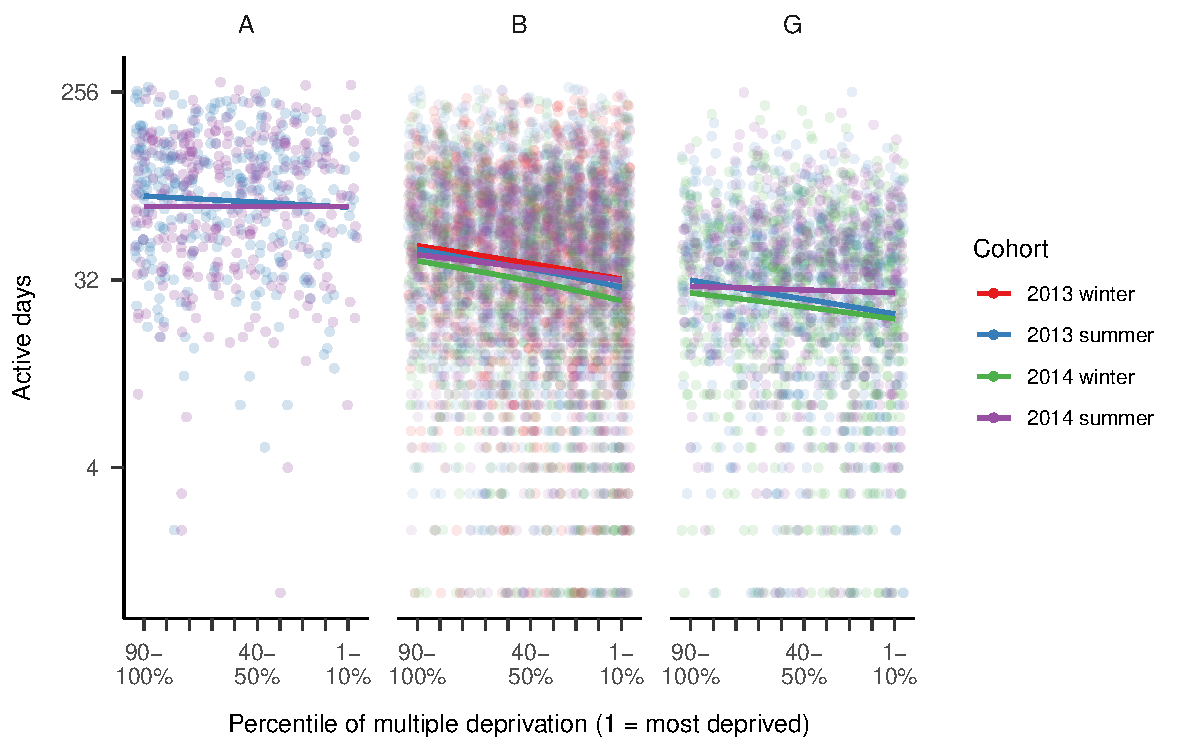
\includegraphics{Assigment-2---OU-data_files/figure-latex/unnamed-chunk-8-1.pdf}
\caption{\label{fig:unnamed-chunk-8}Relationship between VLE activity and assessment results by mode \label{fig:exp6}}
\end{figure}

\hypertarget{discussion}{%
\section{Discussion}\label{discussion}}

The findings presented here highlight that VLE engagement varies widely between students and predicts their module outcomes. Contrary to my expectations based on pedagogical theories, there was no consistent evidence that active engagement was more closely linked to student achievement than passive engagement was. Importantly, the fact that students from disadvantaged backgrounds achieve lower grades, appears likely to be explained in part by lower VLE engagement. These findings have clear implications for my teaching practice. Firstly, they highlight the importance of promoting and monitoring VLE engagement, which can be facilitated by the effective use of learning analytics data like that relied on here. Secondly, they highlight that active learning on VLE platforms needs to be designed in a way that directly furthers learning outcomes and is reflected in subsequent assessments. Thirdly, the achievement of equity in VLE engagement is critical in the path towards removing demographic achievement gaps. In the future, I will experiment with various strategies in the pursuit of that goal, such as the setting and tracking of clear expectations regarding engagement, as well as the provision of VLE resources that seem relevant to all students.

\hypertarget{limitations-and-further-research}{%
\subsection{Limitations and further research}\label{limitations-and-further-research}}

While OULAD is a large dataset that provides insights into actual student behaviours across a range of modules, the available data is limited in several key ways. For one, there is no information regarding the content of the VLE resources, which would be beneficial when it comes to understanding the differential effectiveness of active engagement. Furthermore, there is no measure of `value-add,' but only of overall assessment outcomes. Research into the effectiveness of teaching strategies should be concerned with students' learning over the course of a specific experience, so that knowing more about students' baseline would have allowed for more robust inferences.

Regarding further research with this dataset, I considered only the Social Science modules, as they are of greater relevance to my practice. To understand VLE usage more broadly, the results could be contrasted against the STEM modules also included in that dataset. Similarly, I only considered total VLE engagement over the course of the modules. Further research could consider engagement over time, and thus explore whether there are particularly important turning points. One specific hypothesis worth testing, due to its practical implications, might be that VLE engagement in early days sets students onto a trajectory that becomes difficult to change.

\hypertarget{conclusion}{%
\section{Conclusion}\label{conclusion}}

Online learning environments provide a wealth of data that promises insights into student learning. In this paper, I used a large publicly available data set to explore some key questions regarding the use of virtual learning environments. My findings confirm the value of VLE engagement, highlight the need to carefully design activities that promote active engagement and emphasize the need to consider the risk that VLE usage might exacerbate inequalities. Thus, they will inform my teaching practice. However, the limitations also highlight that research using `big data' must be complemented with deep-dives that consider students' actual engagement with specific online resources.

\newpage

\hypertarget{appendix}{%
\section{Appendix}\label{appendix}}

\begin{figure}
\centering
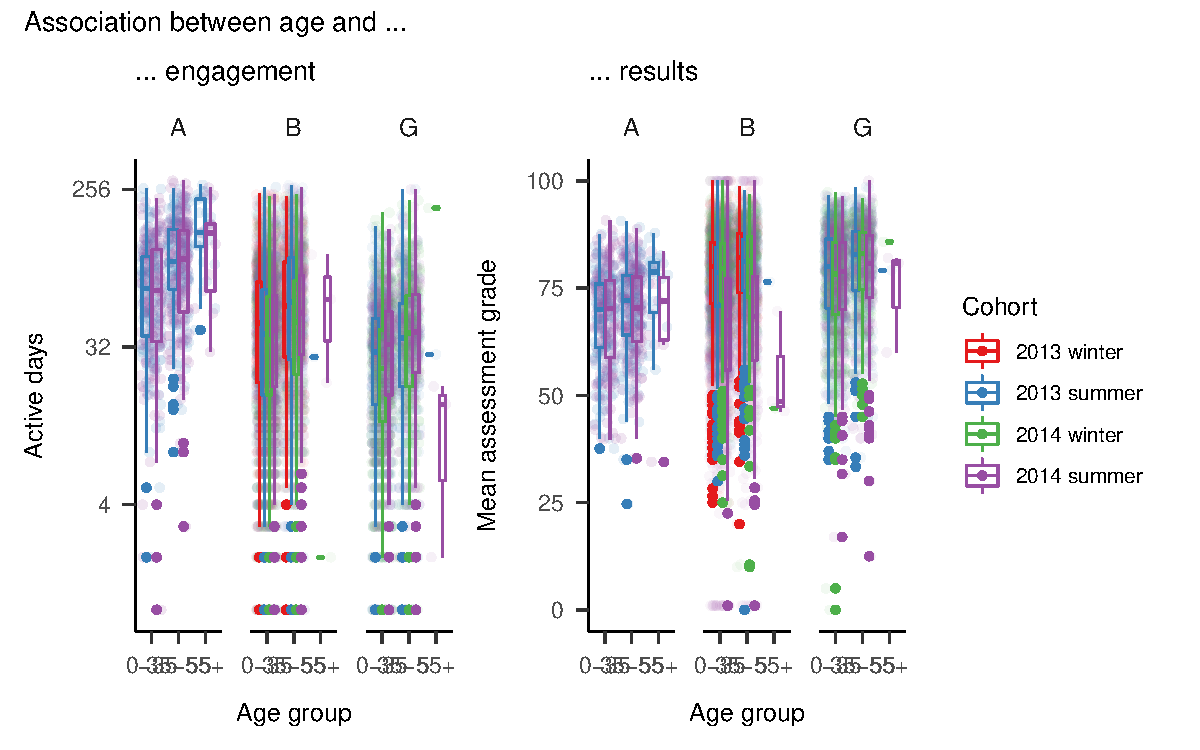
\includegraphics{Assigment-2---OU-data_files/figure-latex/unnamed-chunk-9-1.pdf}
\caption{\label{fig:unnamed-chunk-9}Relationship between age, engagement and outcomes \label{fig:exp7}}
\end{figure}

\newpage

\hypertarget{references}{%
\section{References}\label{references}}

\begingroup
\setlength{\parindent}{-0.5in}
\setlength{\leftskip}{0.5in}

\hypertarget{refs}{}
\begin{CSLReferences}{1}{0}
\leavevmode\hypertarget{ref-R-papaja}{}%
Aust, F., \& Barth, M. (2020). \emph{{papaja}: {Prepare} reproducible {APA} journal articles with {R Markdown}}. Retrieved from \url{https://github.com/crsh/papaja}

\leavevmode\hypertarget{ref-hassan2019virtual}{}%
Hassan, S.-U., Waheed, H., Aljohani, N. R., Ali, M., Ventura, S., \& Herrera, F. (2019). Virtual learning environment to predict withdrawal by leveraging deep learning. \emph{International Journal of Intelligent Systems}, \emph{34}(8), 1935--1952.

\leavevmode\hypertarget{ref-hastie1990generalized}{}%
Hastie, T., \& Tibshirani, R. (1990). Generalized adolitive models. Chapman \& Hall, CRC Press.

\leavevmode\hypertarget{ref-hussain2018student}{}%
Hussain, M., Zhu, W., Zhang, W., \& Abidi, S. M. R. (2018). Student engagement predictions in an e-learning system and their impact on student course assessment scores. \emph{Computational Intelligence and Neuroscience}, \emph{2018}.

\leavevmode\hypertarget{ref-kuzilek2017open}{}%
Kuzilek, J., Hlosta, M., \& Zdrahal, Z. (2017). Open university learning analytics dataset. \emph{Scientific Data}, \emph{4}(1), 1--8.

\leavevmode\hypertarget{ref-R-patchwork}{}%
Pedersen, T. L. (2020). \emph{Patchwork: The composer of plots}. Retrieved from \url{https://CRAN.R-project.org/package=patchwork}

\leavevmode\hypertarget{ref-R-base}{}%
R Core Team. (2021). \emph{R: A language and environment for statistical computing}. Vienna, Austria: R Foundation for Statistical Computing. Retrieved from \url{https://www.R-project.org/}

\leavevmode\hypertarget{ref-sanders2015powered}{}%
Sanders, M., Chonaire, A. N., \& others. (2015). \emph{{``Powered to detect small effect sizes''}: You keep saying that. I do not think it means what you think it means.} The Centre for Market; Public Organisation, University of Bristol, UK.

\leavevmode\hypertarget{ref-smith2015english}{}%
Smith, T., Noble, M., Noble, S., Wright, G., McLennan, D., Plunkett, E., \& others. (2015). The english indices of deprivation 2015. \emph{London: Department for Communities and Local Government}.

\leavevmode\hypertarget{ref-waheed2020predicting}{}%
Waheed, H., Hassan, S.-U., Aljohani, N. R., Hardman, J., Alelyani, S., \& Nawaz, R. (2020). Predicting academic performance of students from VLE big data using deep learning models. \emph{Computers in Human Behavior}, \emph{104}, 106189.

\leavevmode\hypertarget{ref-R-timesaveR}{}%
Wallrich, L. (2021). \emph{timesaveR: Functions to accelerate (academic) data analysis and reporting}. Retrieved from \url{https://lukaswallrich.github.io/timesaveR/}

\leavevmode\hypertarget{ref-R-tidyverse}{}%
Wickham, H., Averick, M., Bryan, J., Chang, W., McGowan, L. D., François, R., \ldots{} Yutani, H. (2019). Welcome to the {tidyverse}. \emph{Journal of Open Source Software}, \emph{4}(43), 1686. \url{https://doi.org/10.21105/joss.01686}

\end{CSLReferences}

\endgroup


\end{document}
